\documentclass[class=book, crop=false, oneside, 12pt]{standalone}
\usepackage{standalone}
\usepackage{../../style}
\usepackage[normalem]{ulem}
\graphicspath{{./assets/images/}}

% arara: pdflatex: { synctex: yes, shell: yes }
% arara: latexmk: { clean: partial }
\begin{document}
\part{Aftermath}
\chapter{La generazione del codice intermedio}
Tiriamo le fila sul compiler frontend

Le fasi sono: an lessicale, distingue I vari lessemi nell'input fornito, in particolare l'output è una stringa di token che deve essere confrontata rispetto al fatto se possa essere generata dalla grammatica considerata; ci sono anche elementi che vengono usati per iniziare  popolare la tabella dei simoli (tipo la roba vista ieri)

An sintattica: fase centrale, in realtà ci sono molte altre attività vengono eseguite al momento del "parsing" (an semantica) 

An semantica: controlli statici, operandi compatibili con gli operatori (magari ho due operatori somma, uno per gli interi e uno per I float; magari posso usarli entrambi, ma devo fare una converisione di tipo). Altri controlli riguardano while e switch statement, magari sono un diobel e ho scritto un break statement;

Dopo tutto questo processo c'è la generazione di codice intermedio, fatta con traduzioni dirette dalla sintassi (schemi di traduzione fatti durante il parsing, non sempre ma spesso)

Cos'è il codice intermedio? È una rappresentazione astratta, abbastanza da non avere tutti I dettagli che trovo nei linguaggi macchina (muovi registro bla bla, illeggibile, vogliamo più astratto), ma deve essere comunque più specifico del linguaggio originale da cui lo abbiamo analizzato

Di solito per la rapp intermedia abbiamo delle possibilità

Abbiamo strutture tipo grafo, come gli AST o un DAG vero e proprio, strutture ottenuto da AST o da parse trees
Dobbiamo immaginare un AST con due foglie, entrambe che rappresentano un identif A, nelDAG avremmo un unico nodo per A e più edge che arrivano alla ehhhh----- insomma I DAG quindi sono più succinti degli AST, che a loro volta sono più succinti dei parse tree
I parse tree sono poco succinti, hanno spesso un botto di cammini lunghi per rappresentare le derivazioni, ma per le operazioni successive sono troppo lenti

Altra possibilità (meglio) è il trhree address code, il nome viene dal fatto che in ciascuna possibile istruzione non possono comparire più di tre indirizzi (e.g. x = y op z)

Terza via è proprio un altro linguaggio, di solito C; questo evita il problema di gestire il backend di compilazione, perché abbiamo già un compilatore per questo linguaggio.
Di solito si usa C perché gcc è figo ed è un linguaggio incredibilmente flessibile

THREE ADDRESS CODE
Rappresentazione linarizzata dei syntax tree, la loro bontà è qui
È una rappresentazione testual- NOOOO ESEMPIO

Passare da ast a three address code
\begin{figure}[H]
    \centering
    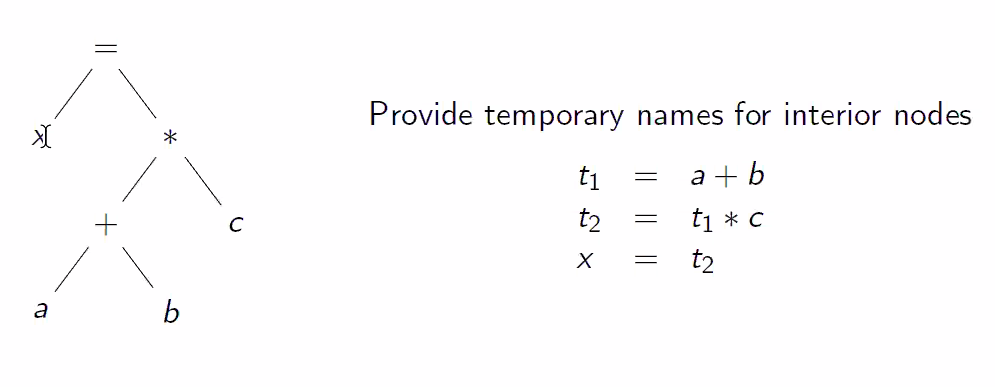
\includegraphics[width=.5\textwidth]{ex1.png}
    \caption{}
    \label{}
\end{figure}
In pratica scorriamo dal basso (?) ed eseguiamo le robe intermedie, salvando in cose temporanee come si vede in figura

Come mai vogliamo la rappresentazione testuale? Mah, vari motivi. In generale diventa molto più semplice fare la generazione di linguaggio macchina oppure operare le ottimizzazioni di questo three address code
È roba che non facciamo ma interessante, parzialmente machine dependent, dipende dal codice macchina su cui stiamo scrivendo il backend

Codice intermedio: esempio
Immaginate che partiamo da 
% img2
Come la traduciamo in codice intermedio?
Una prima approssimazione è questa
% img3
Se x < 100 tutto è vautato come vero (precedenza degli op booleani), quindi vado a L2 (x = 0); altrimenti passo ai controlli successivi che mi portano entrambi a dopo x = 0, altrimeti fannoa nche x = 0
Comunque possiamo fare di meglio
% img4
Controllando se x > 200 è falso possiamo risparmiarci delle etichette e delle righe, sfruttando meglio la corticircuitazione
AHAHAHAHH SE NON È FALSO PASSO A x!=y "PER GRAVITÀ"
Appunto sul fatto che I compilatori sonon furbi perché sfruttano bene la cortocircuitazione? Ok?
Anhce se occhio non è detto che la prima condizione che scriviamo in un'espressione booleana sia la prima a essere valutata

Oggi vediamo come si genera il codice intermedio
Cerchiamo statements di questo tiipo
% img5

P sta per programma e poi kaboom pausa

Allora sì vediamo come fare la trauzione del codice intermedio degli if-then
\begin{figure}[H]
    \centering
    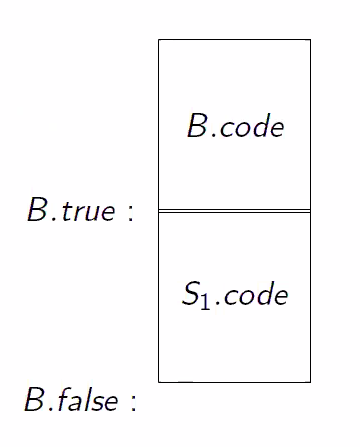
\includegraphics[width=.5\textwidth]{if-then-abstract.png}
    \caption{}
    \label{}
\end{figure}
All'inizio del body del then abbiamo un'etichetta B. true che indica che inizia il body, mentre abbiamo una seconda etichetta B.false che punta alla prima riga successiva al then(?)

Attributi: 
Abbiamo s.next, ereditato, dice qual è la posizione della primissima istruzione di codice da eseguire alla fine di S. teniamo l'etichetta perché s potrebbe essere uno statement composto, potrebbe tenere un while con dentro una catena di if, dobbiamo sempre sapere dopo l'esecuzione del padre
S.code, sintetizzato, andremo a specificare meglio, sequenza di codice intermedio che implementa S
B.true, ereditato, etichetta l'inizio del codice da eseguire se B è vero
Analogamente B.false, dice dove dobbiamo andare se B è falso
B.Code, ereditato, sintetizzato se guardiamo solo l'sdd delle condizioni booleane; è la sequenza dei passi di codice intermedio che implementano la condizione booleana, vanno a b.true se vero e b.false se no

I booleani hanno due funzioni:
Alterare il flusso di controllo
Calcolare dei valori logici nelle espressioni booleani
Il focus di oggi è sulla prima cosa, nella compilazione si distinguono queste due "ortogonali" utilizzi dei booleani, sarebbe anche se utilizzassimo degli interi comme condizioni
% img7
\(P \to S\): il programma è globalmente uno statement
Newlabel() è una funzione che possiamo invocare per la generazione di un'etichetta non ancora utilizzata, mentre triangolo sta per la concatenzione di segmenti di codice intermedio, cioè P.Code è S.code cui si attacca label(S.next); insomma, il codice di è il codice di S a cui è attaccato il riferimento al codice che segue P

S.next = newlabel() è l'inizio dei tempi
È ereditato dal body della produzione iniziale
P.code è sintetizzato, wtf
% img 8
Nell'if-then abbiamo bisognod I una label per B.true, e ok
Ne prendiamo una anche er B.false
Quindi creiamo S.code concatenando il corpo dell'espressione da valutare a label(B.true) e \(S_1.Code\)
Come andiamo a generare bene sta roba?
% img9
% img10
Generiamo una newlable come begin
B.true è una nuovaetichetta
B.false ci porta direttamente a S.next
\(S_1.next\) ci riporta a begin, ovviamente

Quindi come prima cosa label della condizione booleana, poi il codice della condizione; ci mettiamo l'etichetta true, così andiamo al codice, e infine un gen(goto begin) per tornare sopra

% img11
Esempio non completo perché la quaglia è gran puttana

Adesso vediamo la generazione di un or
% img12
% img13
Definiamo true e false
Il codice della b è dato dal codice della \(b_1\), cui segue la label \(B_1.true\), seguito da \(B_2.code\)
Eh vabb sta parte è sfanculata

\end{document}
